% Báo cáo Nhóm 13 trong mẫu IEEE-conference-template-062824.tex của học phần INT3401.
\documentclass[conference]{IEEEtran}
\usepackage{cite}
\usepackage{amsmath,amssymb,amsfonts}
\usepackage{graphicx}
\usepackage{textcomp}
\usepackage{xcolor}
% XeLaTeX và phông Unicode để hiển thị đủ dấu tiếng Việt.
\usepackage{fontspec}
\setmainfont{texgyretermes}[
  Extension=.otf,
  UprightFont=*-regular,
  BoldFont=*-bold,
  ItalicFont=*-italic,
  BoldItalicFont=*-bolditalic]
\usepackage{booktabs}
\usepackage{tabularx}
\usepackage{array}
\usepackage{multirow}
\usepackage[hidelinks]{hyperref}
\usepackage{balance}
\graphicspath{{hinh/}}
% Tên, MSSV và tỷ lệ đóng góp bằng nhau của ba thành viên.
\newcommand{\TenMot}{Đinh Văn Hiến}
\newcommand{\MaMot}{24022986}
\newcommand{\DongGopMot}{33,3\%}
\newcommand{\TenHai}{Nguyễn Thế Ngọc}
\newcommand{\MaHai}{24023046}
\newcommand{\DongGopHai}{33,3\%}
\newcommand{\TenBa}{Nguyễn Văn Thành}
\newcommand{\MaBa}{24023066}
\newcommand{\DongGopBa}{33,3\%}
\newcommand{\KhoMaNguon}{\href{https://github.com/hien20061906-oss/linknopbaiGK_TTNT_-m-i-_-nh-m-13}{GitHub Nhóm 13}}


\begin{document}
\title{Xây dựng và đánh giá các mô hình học máy trong CS188 Project 5}
\author{
\IEEEauthorblockN{\TenMot}
\IEEEauthorblockA{\textit{Mã sinh viên} \MaMot\\INT3401\_10, Nhóm 13}
\and
\IEEEauthorblockN{\TenHai}
\IEEEauthorblockA{\textit{Mã sinh viên} \MaHai\\INT3401\_10, Nhóm 13}
\and
\IEEEauthorblockN{\TenBa}
\IEEEauthorblockA{\textit{Mã sinh viên} \MaBa\\INT3401\_10, Nhóm 13}
}
\maketitle
\renewcommand{\abstractname}{Tóm tắt}
\renewcommand{\figurename}{Hình}
\renewcommand{\tablename}{Bảng}
\renewcommand{\IEEEkeywordsname}{Từ khoá}
\renewcommand{\refname}{Tài liệu tham khảo}

\begin{abstract}
Nhóm triển khai sáu nhiệm vụ trong CS188 Project 5, gồm phân loại nhị phân, hồi quy hàm sin, nhận dạng chữ số bằng hai kiến trúc, nhận diện ngôn ngữ và Attention nhân quả. Bản tích hợp đạt 25/25 điểm trên bộ kiểm thử Berkeley với seed 42. Mạng truyền thẳng đạt 97,94\% trên tập kiểm tra chữ số của Q3 và mạng hồi tiếp đạt 89,20\% trên tập kiểm tra ngôn ngữ. Với Q5, mô hình đạt 94,00\% trên tập đánh giá của bộ chấm và 64,06\% trên tập kiểm tra MNIST tách riêng. Mã nguồn và hướng dẫn chạy được lưu tại \KhoMaNguon.
\end{abstract}
\begin{IEEEkeywords}
Perceptron, hồi quy, MNIST, CNN, RNN, Attention nhân quả
\end{IEEEkeywords}

\begin{table}[!ht]
\caption{Phân công thực hiện của Nhóm 13}
\label{tab:phancong}
\centering\small
\setlength{\tabcolsep}{3pt}
\begin{tabularx}{\columnwidth}{@{}p{0.23\columnwidth}p{0.19\columnwidth}p{0.15\columnwidth}X@{}}
\toprule
Thành viên & MSSV & Đóng góp & Công việc\\
\midrule
\TenMot & \MaMot & \DongGopMot & Q1, Q2, Q6 và demo kiểm thử\\
\TenHai & \MaHai & \DongGopHai & Q3, Q5 và phân tích kết quả ảnh\\
\TenBa & \MaBa & \DongGopBa & Q4 và thực nghiệm nhận diện ngôn ngữ\\
\bottomrule
\end{tabularx}
\end{table}

\section{Giới thiệu và mô tả bài toán}
\subsection{Bài toán và phạm vi thực hiện}
Đề tài dựa trên CS188 Project 5 của Đại học California, Berkeley~\cite{berkeley}. Sáu nhiệm vụ dùng cùng mã khung Python/PyTorch và có cách đánh giá riêng. Q1 nhận một vector đặc trưng và trả nhãn nhị phân. Q2 nhận số thực \(x\) và dự đoán giá trị gần \(\sin(x)\). Q3 và Q5 nhận ảnh chữ số viết tay và trả điểm cho mười lớp từ 0 đến 9. Q4 nhận chuỗi ký tự của một từ và trả điểm cho năm ngôn ngữ. Q6 kiểm tra đầu ra của lớp Attention khi áp dụng mặt nạ nhân quả. Nhóm phân công theo Bảng~\ref{tab:phancong} và tích hợp các phần vào ba tệp \texttt{models.py}, \texttt{train.py} và \texttt{losses.py}.

Mục tiêu thực nghiệm gồm kiểm chứng từng thuật toán, quan sát ảnh hưởng của cấu hình và giải thích những lỗi mô hình còn mắc. Với bài toán phân loại, một giá trị accuracy tổng hợp cho biết tỷ lệ dự đoán đúng, còn ma trận nhầm lẫn cho thấy mô hình thường nhầm giữa những nhãn nào. Với bài toán hồi quy, nhóm theo dõi sai số liên tục và xem đường dự đoán có bám theo giá trị thật trong miền đã học hay không. Riêng Q6, yêu cầu được kiểm chứng bằng giá trị đầu ra, chiều tensor, gradient và tác dụng của mặt nạ.

\subsection{Sản phẩm và tổ chức chương trình}
Sản phẩm của nhóm gồm mã nguồn triển khai Q1--Q6, chương trình kiểm thử, các lệnh demo và kết quả thực nghiệm. Người dùng chọn câu cần chạy để xem điểm kiểm thử, chỉ số đánh giá và hình minh họa. Demo Q4 nhận từ do người dùng nhập rồi trả tên ngôn ngữ dự đoán. Demo Q1, Q2 và Q6 dùng dữ liệu mẫu để minh họa quy tắc phân loại, giá trị hồi quy và tác dụng của mặt nạ Attention. Các kết quả được lưu để đối chiếu với bảng và hình trong báo cáo.

Tệp \texttt{models.py} chứa phép tính từ đầu vào đến dự đoán. Tệp \texttt{losses.py} định nghĩa cách đo sai lệch dùng khi huấn luyện các mạng nơ-ron. Tệp \texttt{train.py} xử lý batch, cập nhật trọng số và, ở các bài phân loại, giữ mô hình có kết quả dev tốt nhất trong lần chạy. Mã khung cung cấp dữ liệu và bộ chấm. Chương trình \path{chay_kiem_thu.py} chạy từng câu với seed đã định, rồi lưu lịch sử và kết quả vào \texttt{ket\_qua/}. Cách tổ chức này cho phép đối chiếu số liệu trong báo cáo với lần chạy tương ứng.

\section{Phương pháp thực hiện}
\subsection{Q1 - Perceptron}
Mô hình tính \(s=\mathbf w^\top\mathbf x\), trả \(+1\) nếu \(s\ge 0\) và trả \(-1\) nếu \(s<0\). Khi dự đoán sai nhãn \(y\), thuật toán cập nhật \(\mathbf w\leftarrow\mathbf w+y\mathbf x\) theo quy tắc Perceptron~\cite{rosenblatt}. Vòng huấn luyện dừng sau một lượt duyệt mà mọi mẫu đều được phân loại đúng. Điều kiện hội tụ gắn với dữ liệu phân tách tuyến tính.

Mã khung sinh 500 điểm có hai đặc trưng \(x_1,x_2\) và gắn nhãn theo dấu của \(x_1+2x_2-1\). Thành phần thứ ba của vector đầu vào luôn bằng 1 để tích vô hướng chứa hệ số chặn. Mỗi lần cập nhật cũng có thể đổi dự đoán của các điểm khác, nên số lỗi qua các lượt có thể tăng tạm thời trước khi về 0.

\subsection{Q2 - Hồi quy hàm sin}
Mạng truyền thẳng \(1\to128\to128\to1\) dùng ReLU ở hai lớp ẩn. Lớp cuối tuyến tính để biểu diễn được cả giá trị âm. Hàm mất mát là \(\mathrm{MSE}=\tfrac1n\sum_i(\hat y_i-y_i)^2\). Nhóm dùng Adam~\cite{adam}, batch 50 và đo MSE trên toàn bộ tập huấn luyện sau mỗi epoch. Cấu hình dùng trong bộ chấm có learning rate \(0{,}003\) và dừng khi MSE không quá \(0{,}005\).

Mã khung tạo 200 giá trị \(x\) cách đều trên \([-2\pi,2\pi]\) và tính nhãn \(y=\sin(x)\). Bình phương làm cho những điểm dự đoán lệch nhiều đóng góp lớn hơn vào MSE. ReLU tạo các đoạn tuyến tính khác nhau trên miền đầu vào, giúp toàn mạng biểu diễn được dạng uốn cong của hàm sin. Nhóm thử ba tốc độ học trong cùng điều kiện khởi tạo để xem cấu hình nào đạt ngưỡng dừng sau ít epoch hơn.

\subsection{Q3 - Nhận dạng chữ số bằng mạng truyền thẳng}
Mạng truyền thẳng nhiều lớp (multilayer perceptron, MLP) được dùng cho Q3. Ảnh MNIST \(28\times28\) được trải phẳng thành vector 784 giá trị~\cite{mnist}. Mạng \(784\to200\to10\) dùng ReLU ở lớp ẩn. Lớp cuối trả logits. Cross-entropy dùng logits trong huấn luyện và \(\arg\max\) chọn lớp khi dự đoán. Nhóm dùng Adam với learning rate \(0{,}001\), batch 100, lưu trọng số có độ chính xác dev cao nhất và dừng khi dev đạt 98\% hoặc đủ 30 epoch.

Với một batch gồm \(B\) ảnh, mô hình nhận tensor \(B\times784\) và trả tensor \(B\times10\). Mỗi hàng chứa mười điểm thô của một ảnh. Cross-entropy kết hợp chuẩn hóa và lấy log xác suất của lớp thật bên trong hàm mất mát. Bởi vậy, đầu ra tuyến tính được đưa trực tiếp vào hàm này. Phép trải phẳng vẫn giữ giá trị và vị trí cố định của từng điểm ảnh, còn lớp kết nối đầy đủ học trọng số riêng cho từng tọa độ.

\subsection{Q4 - Nhận diện ngôn ngữ bằng RNN}
Mạng nơ-ron hồi tiếp (recurrent neural network, RNN) được dùng cho Q4. Mỗi ký tự được mã hóa one-hot trên bảng chữ cái 47 phần tử. Mạng duyệt tuần tự, kết hợp ký tự hiện tại \(x_t\) và trạng thái trước \(h_{t-1}\) để tạo trạng thái mới:
\[
h_t=\operatorname{ReLU}(W_x x_t+b_x+W_h h_{t-1}+b_h).
\]
Ký tự đầu khởi tạo trạng thái bằng nhánh \(W_x\). Mô hình giữ nguyên trạng thái tại vị trí đệm. Lớp cuối ánh xạ trạng thái ẩn 192 chiều sang năm logits. Nhóm gom từ cùng độ dài, xáo nhóm và mẫu, dùng Adam với learning rate \(0{,}002\), batch tối đa 128 và 20 epoch. Gradient được giới hạn chuẩn ở 5. Trọng số được chọn theo dev trước khi đánh giá test.

Năm nhãn lần lượt là tiếng Anh, Tây Ban Nha, Phần Lan, Hà Lan và Ba Lan. Mỗi bước hồi tiếp dùng cùng bộ trọng số. Trạng thái \(h_{t-1}\) mang thông tin từ các ký tự trước nên hai từ có cùng nhóm ký tự nhưng khác thứ tự vẫn có thể cho trạng thái cuối khác nhau. Việc gom các từ cùng độ dài giúp xử lý nhiều mẫu trong một batch. Bước giới hạn chuẩn gradient giảm mức cập nhật khi gradient qua chuỗi tăng quá lớn.

\subsection{Q5 - Nhận dạng chữ số bằng CNN}
Mạng nơ-ron tích chập (convolutional neural network, CNN) được dùng cho Q5. Hàm \texttt{Convolve} trượt kernel qua ảnh với bước 1, nhân từng phần tử và cộng trong mỗi cửa sổ. Kernel \(3\times3\) cho bản đồ đặc trưng \(26\times26\) khi áp dụng lên ảnh \(28\times28\) không chèn viền. Bản đồ đặc trưng được trải phẳng, đi qua lớp ẩn 100 nút và lớp cuối 10 logits. Nhóm huấn luyện bằng cross-entropy, Adam với learning rate \(0{,}001\) và batch 50. Bộ trọng số có dev cao nhất được dùng cho hai phép đánh giá.

Với ảnh \(X\) và kernel \(K\) kích thước \(h\times w\), phần tử bản đồ đặc trưng tại hàng \(i\), cột \(j\) được tính như sau:
\[
Z_{ij}=\sum_{a=0}^{h-1}\sum_{b=0}^{w-1}K_{ab}X_{i+a,j+b}.
\]
Chẳng hạn, cửa sổ \(\bigl[\begin{smallmatrix}1&2\\4&5\end{smallmatrix}\bigr]\) và kernel \(\bigl[\begin{smallmatrix}1&0\\0&1\end{smallmatrix}\bigr]\) cho một ô bằng \(1+5=6\). Các vị trí dùng chung hệ số kernel. Bản đồ có \(26^2=676\) giá trị trước khi đi vào các lớp kết nối đầy đủ. Trong lần chạy được báo cáo, mô hình dừng sau epoch thứ hai khi dev đạt 86\%, vượt ngưỡng dừng 85\%.

\subsection{Q6 - Attention nhân quả}
Ba phép chiếu tuyến tính tạo \(Q\), \(K\) và \(V\) từ đầu vào. Lớp tính
\[
\operatorname{softmax}\!\left(QK^\top/\sqrt{d_k}+M\right)V,
\]
trong đó \(M_{ij}=0\) nếu \(j\le i\) và \(M_{ij}=-\infty\) nếu \(j>i\). Softmax chuẩn hóa theo chiều các vị trí khóa, nên trọng số vị trí tương lai bằng 0~\cite{attention}. Với đầu vào kích thước \(B\times T\times d_k\), ma trận điểm có kích thước \(B\times T\times T\) và đầu ra có kích thước \(B\times T\times d_k\).

Mỗi hàng của ma trận điểm biểu diễn mức liên quan giữa một vị trí truy vấn và tất cả vị trí khóa. Phép chia cho \(\sqrt{d_k}\) giữ thang độ lớn của tích vô hướng khi số chiều tăng. Sau khi che các vị trí tương lai, softmax phân bổ trọng số cho những vị trí còn lại. Tại vị trí đầu tiên, chỉ có một vị trí hợp lệ nên trọng số tại đó bằng 1. Tại các vị trí sau, đầu ra là tổng có trọng số của các vector \(V\) đã được phép sử dụng.

\section{Thiết lập thực nghiệm}
Nhóm chạy trên CPU, Python 3.12, PyTorch 2.15.0+cpu và NumPy 1.26.4. Lệnh kiểm thử chạy từng câu trong một tiến trình riêng với seed 42. Q1 và Q2 dùng dữ liệu sinh bởi mã khung. Q2 có thêm 199 điểm nằm giữa các cặp mẫu huấn luyện liền kề để đo nội suy trong cùng miền \(x\).

\begin{table}[!t]
\caption{Các tập dữ liệu và vai trò trong thực nghiệm}
\label{tab:dulieu}
\centering\small
\setlength{\tabcolsep}{4pt}
\begin{tabularx}{\columnwidth}{@{}l>{\raggedright\arraybackslash}p{0.24\columnwidth}X@{}}
\toprule
Câu & Huấn luyện & Chọn mô hình và đánh giá\\
\midrule
Q1 & 500 điểm sinh & Kiểm tra lỗi trên tập huấn luyện\\
Q2 & 200 điểm trên miền sin & MSE train và 199 điểm nội suy\\
Q3 & 60.000 ảnh & 5.000 ảnh dev, 5.000 ảnh test\\
Q4 & 17.500 từ & 500 từ dev, 500 từ test\\
Q5 & 200 ảnh & 50 ảnh dev và 50 ảnh bộ chấm nằm trong train. Đo thêm trên 10.000 ảnh test riêng\\
Q6 & --- & Kiểm tra toán học trên tensor mẫu\\
\bottomrule
\end{tabularx}
\end{table}

\subsection{Chia dữ liệu và chọn trọng số}
Bảng~\ref{tab:dulieu} cho biết dữ liệu dùng ở từng bước. Tập train dùng để cập nhật trọng số. Tập dev dùng để chọn epoch hoặc quyết định khi nào dừng. Với Q3, tập kiểm tra MNIST gốc gồm 10.000 ảnh được chia xen kẽ theo chỉ số chẵn và lẻ thành hai phần bằng nhau. Với Q4, bộ dữ liệu ngôn ngữ đã cung cấp ba tập riêng. Sau khi chọn bộ trọng số theo dev, nhóm dùng tập test để báo cáo kết quả cuối.

Trong mã khung Q5, 100 ảnh đầu của tập huấn luyện MNIST được chia theo chỉ số chẵn và lẻ làm dev và test của bộ chấm. Cả 100 ảnh đồng thời thuộc 200 ảnh train Q5. Nhóm thực hiện thêm phép đo trên 10.000 ảnh của tập test MNIST gốc, giữ nguyên mô hình và không dùng ảnh test này để chọn trọng số.

\subsection{Chỉ số và cách kiểm tra lại}
Accuracy là số mẫu dự đoán đúng chia cho tổng số mẫu. Trong ma trận nhầm lẫn, hàng là nhãn thật, cột là nhãn dự đoán. Các ô trên đường chéo là dự đoán đúng. Khi muốn xem một lớp riêng, nhóm lấy số đúng trên đường chéo chia cho tổng số mẫu của hàng đó. Q2 dùng MSE thay cho accuracy vì đầu ra là số thực. Q6 dùng bộ chấm của đề, đối chiếu công thức với PyTorch và kiểm tra gradient.

Có thể dùng \path{chuan_bi_du_lieu.py} trong thư mục \path{cong_cu} để lấy dữ liệu, sau đó chạy lệnh \texttt{python chay\_kiem\_thu.py all --seed 42}. Nhật ký ghi điểm từng câu. Tùy chọn \texttt{--phan-tich} cho Q3, Q4 hoặc Q5 tạo ma trận nhầm lẫn và các minh họa tương ứng. Gói nộp giữ mã nguồn và log thực nghiệm. README hướng dẫn lấy lại dữ liệu gốc khi cần chạy.



\section{Kết quả và phân tích}
Bảng~\ref{tab:ketqua} tổng hợp chỉ số thực nghiệm và điểm bộ kiểm thử Berkeley. Phép kiểm tra độc lập chép ba tệp Python từ gói nộp vào mã khung nguyên bản cũng đạt 25/25 với seed 42.

\begin{table}[!t]
\caption{Kết quả bản tích hợp với seed 42}
\label{tab:ketqua}
\centering\small
\setlength{\tabcolsep}{4pt}
\begin{tabularx}{\columnwidth}{@{}l>{\raggedright\arraybackslash}p{0.18\columnwidth}X@{}}
\toprule
Câu & Điểm Berkeley & Chỉ số thực nghiệm\\
\midrule
Q1 & 5/5 & 500/500 mẫu huấn luyện đúng trong demo\\
Q2 & 5/5 & MSE huấn luyện 0,003010\\
Q3 & 5/5 & 4.897/5.000 ảnh test (97,94\%)\\
Q4 & 5/5 & 446/500 từ test (89,20\%)\\
Q5 & 3/3 & 47/50 ảnh bộ chấm (94,00\%), 6.406/10.000 ảnh test riêng (64,06\%)\\
Q6 & 2/2 & Đầu ra khớp tham chiếu, vượt kiểm tra mặt nạ và gradient\\
\midrule
Tổng & 25/25 & \\
\bottomrule
\end{tabularx}
\end{table}

\subsection{Q1 - Số lỗi qua các lượt huấn luyện}
Trong demo Q1, các seed 0, 42 và 73 dừng sau 5, 22 và 3 lượt duyệt. Cả ba phân loại đúng 500/500 mẫu huấn luyện tương ứng. Số lượt hội tụ phụ thuộc vào dữ liệu sinh và thứ tự cập nhật. Với mẫu minh họa \(\mathbf x=[2,1,1]\) ở seed 42, mô hình cho điểm xấp xỉ \(23{,}72\) và dự đoán \(+1\). Quy tắc sinh nhãn cũng cho \(+1\), vì \(2+2\cdot1-1=3>0\).

\begin{figure}[!ht]
\centering
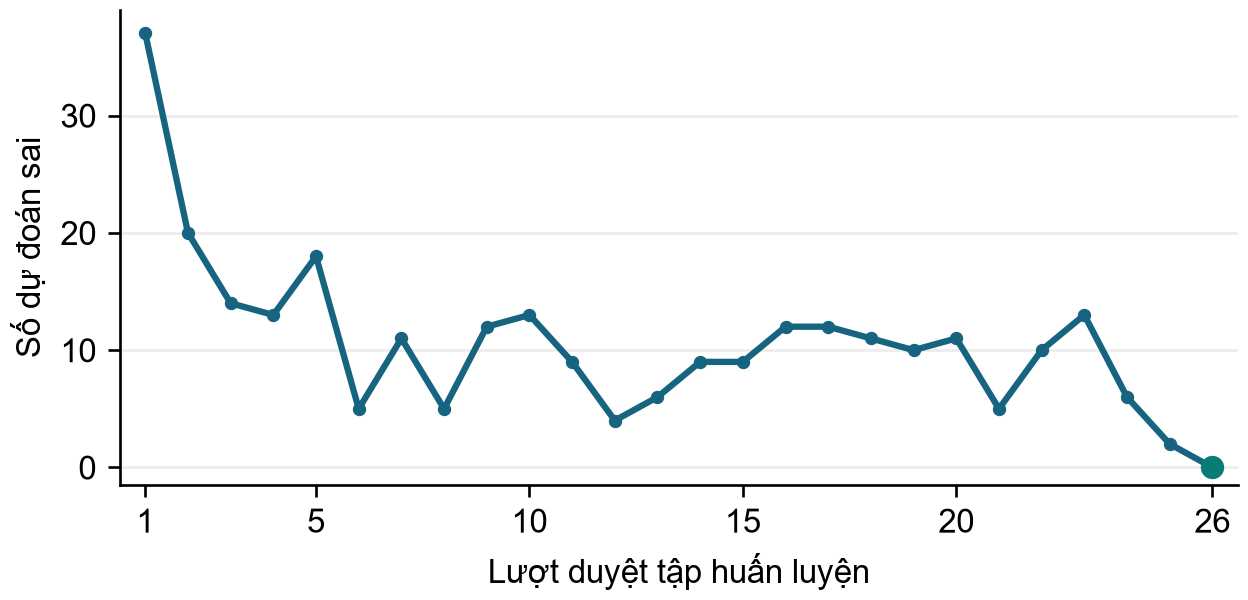
\includegraphics[width=\columnwidth]{q1_so_loi.png}
\caption{Số lần dự đoán sai trong mỗi lượt duyệt của Q1, lấy từ lần chạy bộ kiểm thử seed 42.}
\label{fig:q1}
\end{figure}

Hình~\ref{fig:q1} là nhật ký của bộ kiểm thử, một lần chạy riêng với demo. Số lỗi giảm từ 37 ở lượt đầu xuống 0 ở lượt 26, đồng thời có các đoạn tăng ngắn, chẳng hạn từ 13 lên 18 ở lượt 4–5. Đại lượng này đếm các sai sót xảy ra trong lúc trọng số đang được cập nhật. Lượt cuối có 0 lỗi cho thấy mô hình hoàn thành một lượt mà không cần cập nhật thêm.

\subsection{Q2 - Ảnh hưởng của tốc độ học}

\begin{table}[!t]
\caption{Thử tốc độ học ở Q2 với seed 42}
\label{tab:q2}
\centering\small
\begin{tabular}{@{}rrrr@{}}
\toprule
Learning rate & Epoch & MSE train & MSE nội suy\\
\midrule
0,001 & 119 & 0,004957 & 0,004582\\
0,003 & 83 & 0,003010 & 0,002811\\
0,005 & 85 & 0,004201 & 0,003917\\
\bottomrule
\end{tabular}
\end{table}

Ở Q2, Bảng~\ref{tab:q2} cho thấy \(0{,}003\) đạt ngưỡng dừng sớm nhất trong ba cấu hình và có MSE nội suy thấp nhất trong phép thử này. Với \(x=1\), mô hình cho \(0{,}8220\) so với \(\sin(1)\approx0{,}8415\). Kết quả mô tả nội suy trong miền đã huấn luyện. Hình~\ref{fig:q2} biểu diễn đường dự đoán và MSE qua các epoch.

\begin{figure*}[!t]
\centering
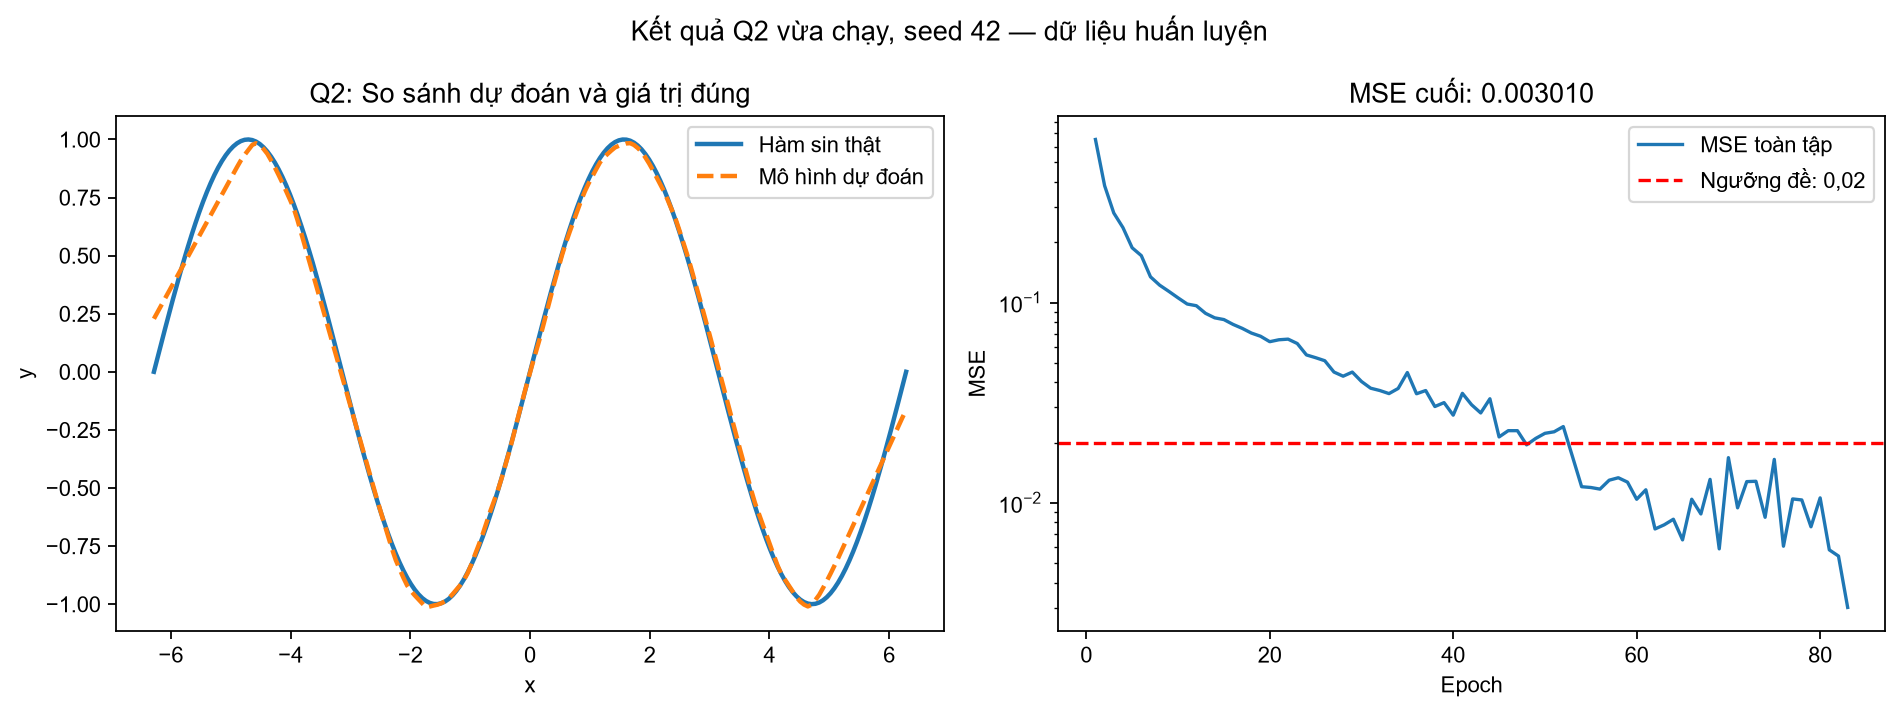
\includegraphics[width=0.87\textwidth]{q2_seed42_bieu_do.png}
\caption{Q2 với learning rate 0,003. Hình trái so sánh đường dự đoán với hàm sin thật. Hình phải theo dõi MSE huấn luyện qua từng epoch.}
\label{fig:q2}
\end{figure*}

Đường dự đoán bám dạng tuần hoàn trong miền quan sát và còn lệch ở một số đoạn gần biên. MSE \(0{,}003010\) thấp hơn mức \(0{,}02\) của bộ chấm. Mỗi cấu hình trong Bảng~\ref{tab:q2} được dừng khi đạt cùng ngưỡng MSE train, nên số epoch phản ánh tốc độ đạt mục tiêu của lần chạy. Ba phép thử cùng seed chưa đủ để kết luận một tốc độ học luôn tốt nhất. Kết quả nội suy cũng chưa đánh giá dự đoán ngoài \([-2\pi,2\pi]\).

\subsection{Q3 - Cấu hình MLP và các ảnh bị nhầm}
Nhóm khảo sát hai kiến trúc lớp ẩn bằng ba seed, cùng learning rate \(0{,}001\) và batch 100. Bảng~\ref{tab:q3cauhinh} dùng accuracy ở epoch cuối trên dev của các lần khảo sát. Mạng hai lớp ẩn có trung bình cao hơn khoảng 0,05 điểm phần trăm, nhưng thứ tự thay đổi theo seed. Kết quả này chưa cho thấy lợi thế ổn định của việc thêm lớp. Bản tích hợp dùng mạng một lớp ẩn với 200 nút, có ít tham số hơn.

\begin{table}[!ht]
\caption{Accuracy dev tại epoch cuối trong khảo sát Q3}
\label{tab:q3cauhinh}
\centering\small
\setlength{\tabcolsep}{4pt}
\begin{tabular}{@{}lrrrr@{}}
\toprule
Lớp ẩn & Seed 0 & Seed 1 & Seed 2 & TB\\
\midrule
200 & 97,74\% & 97,90\% & 97,92\% & 97,85\%\\
200 và 100 & 98,22\% & 97,70\% & 97,78\% & 97,90\%\\
\bottomrule
\end{tabular}
\end{table}

Trong lần kiểm thử tích hợp seed 42, accuracy dev tăng từ 94,74\% ở epoch 1 lên 98,02\% ở epoch 10. Mô hình đúng 4.897 trong 5.000 ảnh test. Trong ma trận nhầm lẫn, 9 bị đoán thành 4 là lỗi theo cặp phổ biến nhất với 7 trường hợp. Tổng cộng mô hình nhận đúng 467/485 ảnh nhãn 9, tức 96,29\%. Đây là lớp có tỷ lệ nhận đúng thấp nhất trong lần kiểm tra. Hình~\ref{fig:mnist} cho thấy ví dụ của Q3 và Q5. Nhãn thật đứng trước mũi tên và dự đoán đứng sau mũi tên.

\begin{figure*}[!t]
\centering
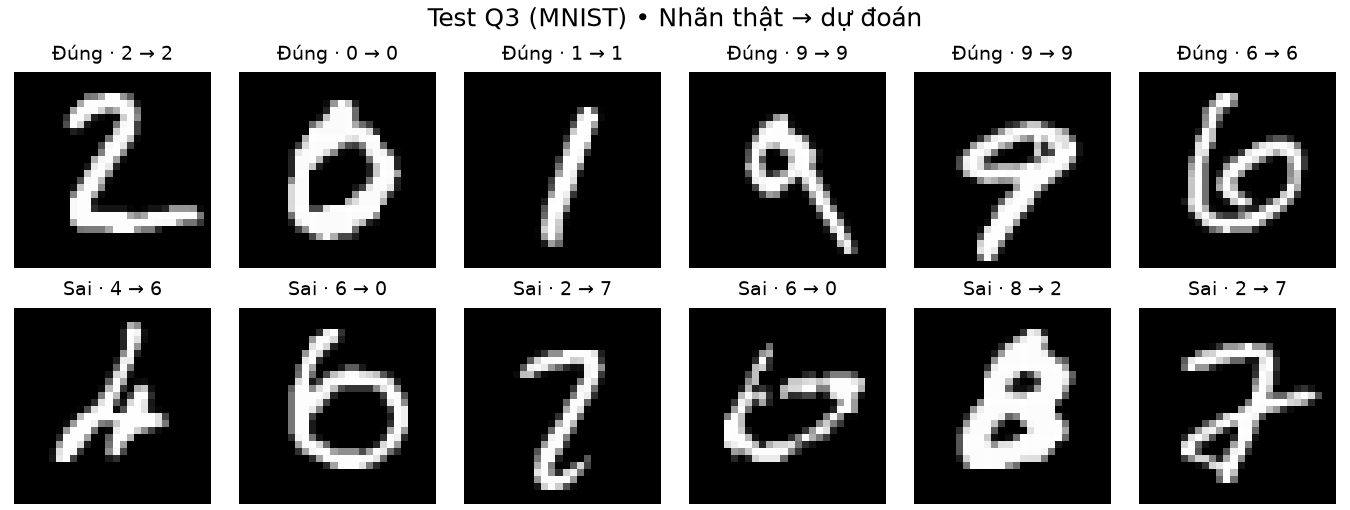
\includegraphics[width=0.47\textwidth]{q3_seed42_vi_du.png}
\hfill
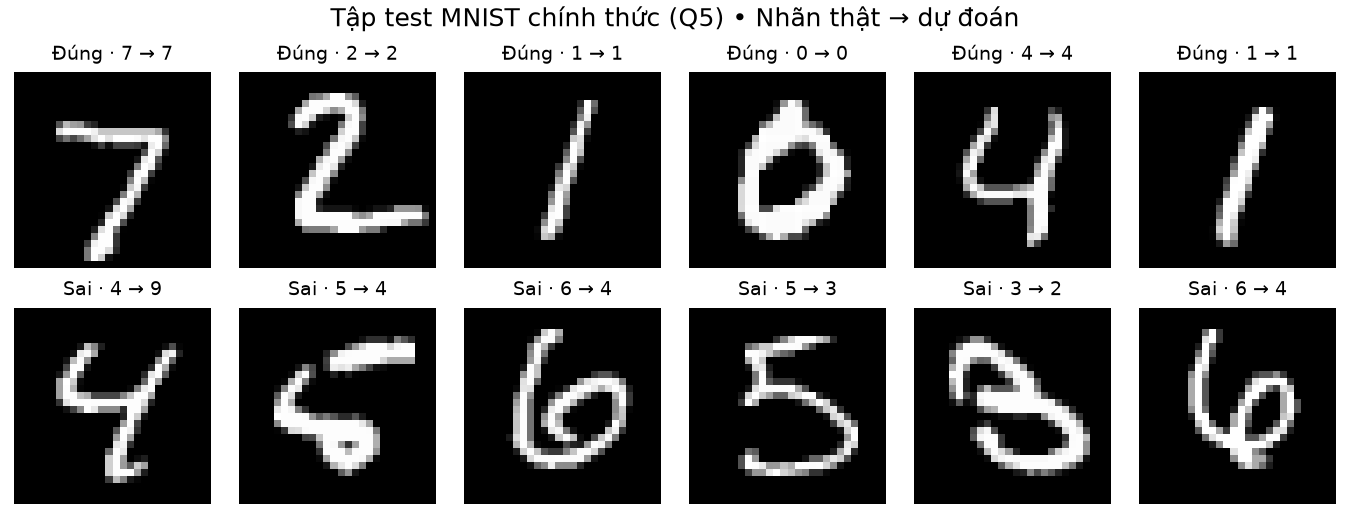
\includegraphics[width=0.47\textwidth]{q5_seed42_vi_du.png}
\caption{Ảnh chữ số và dự đoán của Q3 (trái) và Q5 (phải). Hàng trên gồm các mẫu đúng, hàng dưới gồm các mẫu sai. Hai phần dùng tập test tương ứng với từng câu.}
\label{fig:mnist}
\end{figure*}

\subsection{Q4 - Lựa chọn kích thước trạng thái và phân tích lỗi}
Ở giai đoạn khảo sát, nhóm thử bốn cặp kích thước trạng thái ẩn và tốc độ học trên cùng tập dev. Mỗi cấu hình trong Bảng~\ref{tab:q4cauhinh} chạy 12 epoch với seed 42. Mức 192 nút và tốc độ học \(0{,}002\) đạt kết quả dev cao nhất trong phép sàng lọc. Các lần lặp riêng với 20 epoch cho accuracy dev tốt nhất từ 90,20\% đến 91,80\%. Bảng dùng log khảo sát. Các kết quả trong Bảng~\ref{tab:ketqua} lấy từ bản tích hợp huấn luyện lại.

\begin{table}[!ht]
\caption{Accuracy dev tốt nhất trong khảo sát Q4, seed 42}
\label{tab:q4cauhinh}
\centering\small
\begin{tabular}{@{}rrr@{}}
\toprule
Số nút ẩn & Learning rate & Accuracy dev\\
\midrule
64  & 0,002 & 85,40\%\\
128 & 0,001 & 87,60\%\\
128 & 0,002 & 88,80\%\\
192 & 0,002 & 91,00\%\\
\bottomrule
\end{tabular}
\end{table}

Bản tích hợp đạt 90,80\% trên dev tại epoch 16 và đạt 89,20\% trên test sau khi khôi phục trọng số của epoch đó. Hình~\ref{fig:q4cm} cho thấy mỗi ngôn ngữ có 100 từ test. Tiếng Phần Lan được nhận đúng 94/100 từ, còn tiếng Hà Lan được nhận đúng 83/100 từ. Có 13 từ tiếng Hà Lan bị dự đoán thành tiếng Anh, chiếm 13 trong 54 lỗi trên test. Theo chiều ngược lại, 6 từ tiếng Anh bị dự đoán thành tiếng Hà Lan. Hai số này cho biết lỗi theo từng hướng và giúp chọn cặp nhãn để khảo sát tiếp.

\begin{figure}[!ht]
\centering
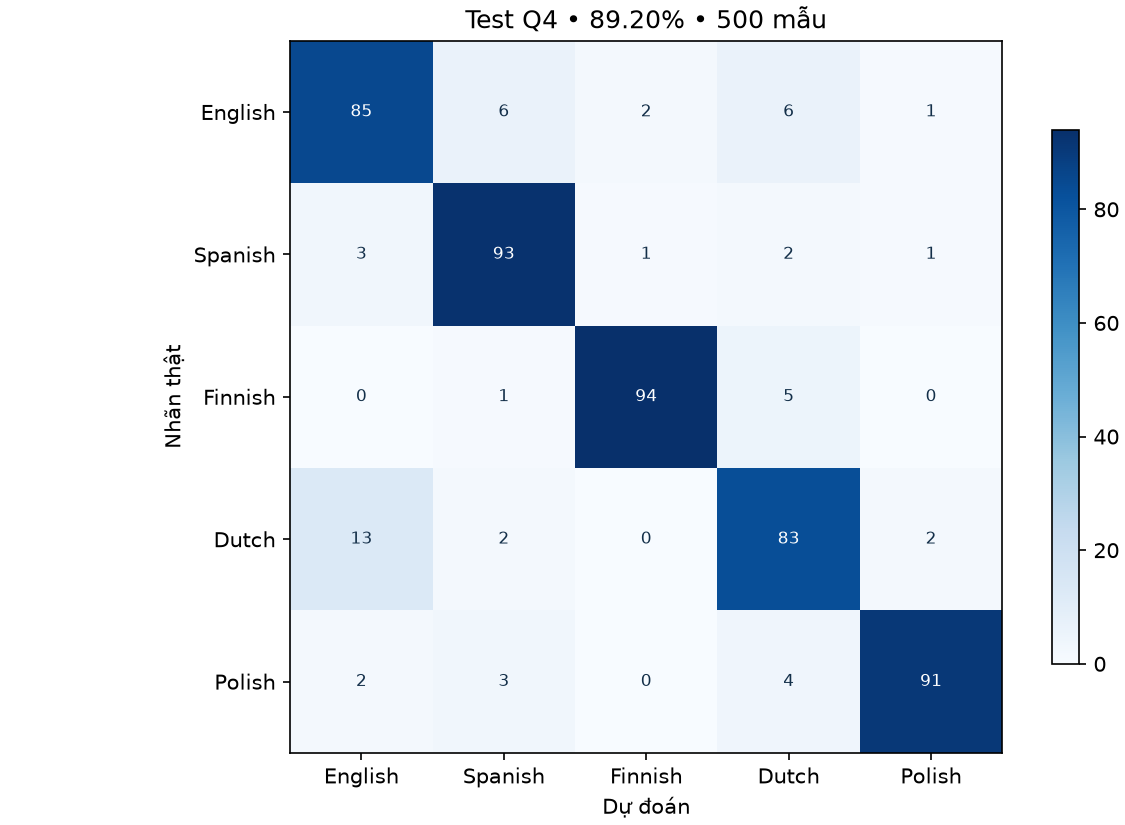
\includegraphics[width=\columnwidth]{q4_seed42_ma_tran.png}
\caption{Ma trận nhầm lẫn Q4 trên 500 từ test. Hàng biểu thị nhãn thật và cột biểu thị dự đoán.}
\label{fig:q4cm}
\end{figure}

Trong demo nhập từ, mô hình đoán đúng \textit{kiitos} là tiếng Phần Lan và đoán \textit{hello} thành tiếng Phần Lan. Những ví dụ đơn lẻ giúp thấy dạng đầu vào và đầu ra. Tỷ lệ đúng trên tập test mới phản ánh kết quả trên toàn bộ mẫu được đánh giá.

\subsection{Q5 - Chênh lệch giữa hai tập đánh giá}
Sau hai epoch, loss trung bình trên tập train giảm từ \(2{,}0253\) xuống \(1{,}2405\), còn accuracy dev tăng từ 72\% lên 86\%. Mô hình đạt 94,00\% trên 50 ảnh của bộ chấm và 64,06\% trên tập test MNIST tách riêng. Mức 64,06\% phản ánh độ chính xác trên ảnh chưa dùng để học hoặc chọn trọng số. Chênh lệch 29,94 điểm phần trăm cho thấy kết quả nhạy với cách lấy mẫu đánh giá. Do quy mô và mức trùng dữ liệu khác nhau, hai phép đo trả lời các câu hỏi khác nhau về cùng bộ trọng số.

\begin{figure}[!ht]
\centering
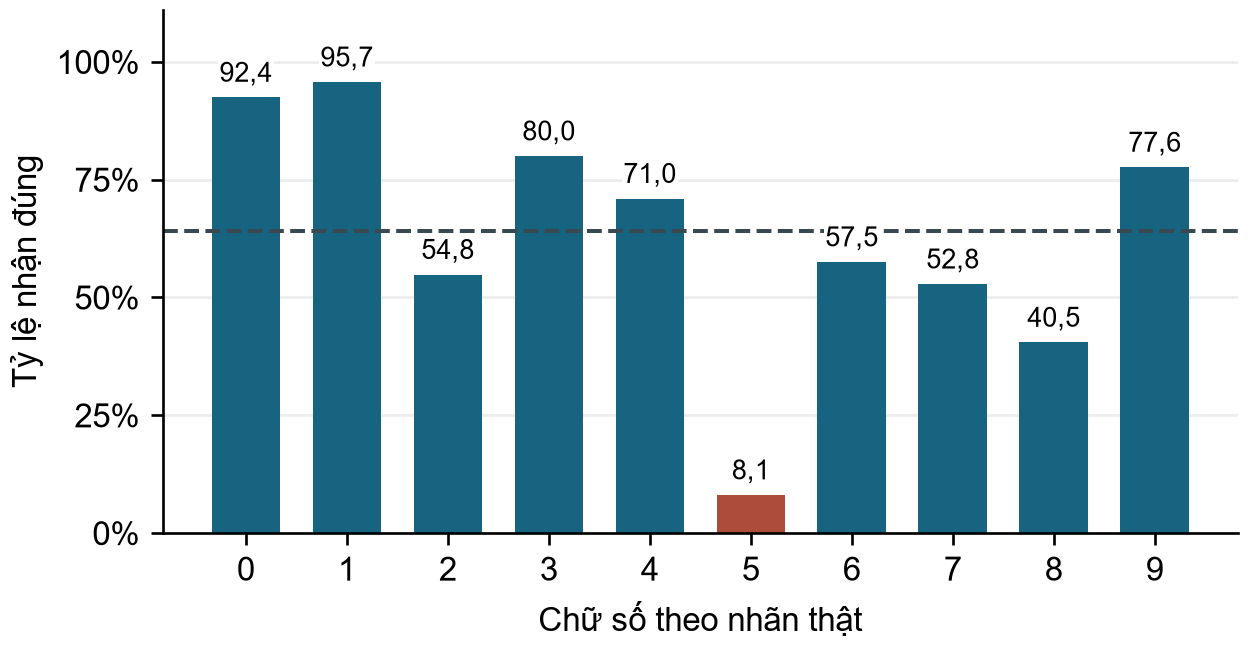
\includegraphics[width=\columnwidth]{q5_ty_le_theo_chu_so.png}
\caption{Tỷ lệ nhận đúng theo nhãn thật trên 10.000 ảnh MNIST test riêng của Q5. Đường đứt là accuracy chung trên tất cả ảnh.}
\label{fig:q5lop}
\end{figure}

Hình~\ref{fig:q5lop} cho thấy mức sai khác lớn giữa các lớp. Mô hình nhận đúng 1.086/1.135 ảnh số 1, đạt 95,68\%, nhưng chỉ đúng 72/892 ảnh số 5, đạt 8,07\%. Có 317 ảnh số 5 bị dự đoán thành số 3. Tập huấn luyện 200 ảnh chỉ có 13 ảnh số 5. Đây là một dấu hiệu để thiết kế phép thử tiếp theo với nhiều ảnh hơn và số mẫu mỗi lớp cân bằng hơn. Thí nghiệm hiện tại chưa tách riêng ảnh hưởng của số mẫu, độ đa dạng nét viết và cấu trúc mạng.

\balance
\subsection{Q6 - Kiểm tra tính nhân quả}
Trong demo Q6, nhóm dùng ba phép chiếu đồng nhất để quan sát trực tiếp tác dụng của mặt nạ. Đầu vào có ba token \([1,0]\), \([0,1]\) và \([1,1]\). Nhóm đổi token thứ ba thành \([11,11]\) rồi chạy lại. Bảng~\ref{tab:q6demo} ghi đầu ra trước và sau khi đổi. Hai vị trí đầu giữ nguyên vì mặt nạ chặn vị trí 3 ở các hàng tương ứng. Vị trí 3 được dùng chính token vừa đổi, nên đầu ra ở vị trí đó thay đổi.

\begin{table}[!ht]
\caption{Đầu ra Q6 khi đổi token cuối}
\label{tab:q6demo}
\centering\small
\begin{tabular}{@{}lll@{}}
\toprule
Vị trí & Trước khi đổi & Sau khi đổi\\
\midrule
1 & \([1,0]\) & \([1,0]\)\\
2 & \([0{,}330\quad 0{,}670]\) & \([0{,}330\quad 0{,}670]\)\\
3 & \([0{,}752\quad 0{,}752]\) & \([11,11]\)\\
\bottomrule
\end{tabular}
\end{table}

Kiểm thử bổ sung đối chiếu đầu ra với phép Attention tham chiếu của PyTorch trên nhiều kích thước batch và chiều dài chuỗi. Nhóm kiểm tra cả gradient và điều kiện đầu ra ở các vị trí trước giữ nguyên khi token cuối thay đổi. Phép kiểm tra này đánh giá một khối Attention nhân quả độc lập.

\section{Giới hạn của thực nghiệm}
Các lần kiểm thử chính dùng một seed để có thể chạy lại và đối chiếu kết quả. Khảo sát nhiều seed của Q1, Q3 và Q4 cung cấp thêm thông tin về độ dao động trong cấu hình đã thử. Phạm vi kết luận vẫn gắn với mã khung và dữ liệu đang dùng. Ở Q4, mô hình học từ đơn trong năm ngôn ngữ với bảng ký tự cố định. Đánh giá này chưa bao quát câu dài, từ trộn nhiều ngôn ngữ hoặc ký tự ngoài bảng chữ cái.

Muốn so sánh MLP và CNN theo kiến trúc, cần huấn luyện trên cùng tập dữ liệu, dùng cùng tập dev và đánh giá trên cùng một tập test rời. Trong bài này, Q3 học trên 60.000 ảnh còn Q5 học trên 200 ảnh, nên mỗi accuracy mô tả một thiết lập riêng. Với Q2, bước đánh giá tiếp theo có thể tách miền nội suy và miền ngoại suy. Với Q6, mục tiêu của phép thử là xác nhận phép tính và mặt nạ trong phạm vi lớp đã cài đặt.

\section{Kết luận}
Nhóm đã tích hợp sáu nhiệm vụ và đối chiếu kết quả với bộ chấm Berkeley. Khảo sát Q2 làm rõ tốc độ đạt ngưỡng MSE ở ba tốc độ học. Ma trận nhầm lẫn Q3 và Q4 cho thấy những nhãn cần xem xét thêm. Phép đo bổ sung ở Q5 cho thấy vai trò của tập test tách riêng. Demo Q6 minh họa tính nhân quả bằng cách thay đổi token cuối và kiểm tra các đầu ra trước đó. Log, ảnh dự đoán, ma trận nhầm lẫn và hướng dẫn trong gói mã nguồn cho phép kiểm tra lại các kết quả đã báo cáo.

\begin{thebibliography}{00}
\bibitem{berkeley} University of California, Berkeley, \emph{CS 188 Fall 2025, Project 5: Machine Learning}. [Trực tuyến]. Địa chỉ \url{https://inst.eecs.berkeley.edu/~cs188/archive/fa25/projects/proj5/}.
\bibitem{rosenblatt} F. Rosenblatt, \emph{The perceptron: A probabilistic model for information storage and organization in the brain}, Psychological Review, tập 65, số 6, tr. 386--408, 1958, doi: 10.1037/h0042519.
\bibitem{adam} D. P. Kingma và J. Ba, \emph{Adam: A Method for Stochastic Optimization}, Proc. ICLR, 2015. [Trực tuyến]. Địa chỉ \url{https://arxiv.org/abs/1412.6980}.
\bibitem{mnist} Y. LeCun, L. Bottou, Y. Bengio và P. Haffner, \emph{Gradient-based learning applied to document recognition}, Proceedings of the IEEE, tập 86, số 11, tr. 2278--2324, 1998, doi: 10.1109/5.726791.
\bibitem{attention} A. Vaswani và cộng sự, \emph{Attention Is All You Need}, Advances in Neural Information Processing Systems, tập 30, 2017. [Trực tuyến]. Địa chỉ \url{https://arxiv.org/abs/1706.03762}.
\end{thebibliography}
\end{document}
